\section{Comparison with Dijkstra}\label{sec:comparison}

The Dijkstra algorithm tries to find a minimum \emph{spanning} tree which
contains links that connect a set of target nodes.

Differently from that, the minimum \emph{Steiner} tree considers for the
computations, to connect all the target nodes, also other nodes. So in this way
the lower bound of the optimal solution is less or equal than the result
provided by a \emph{spanning} tree algorithm (as we can see in
\figref{fig:steiner}). The price to pay is in term of time and computational
power, because the algorithm has to visit all the possible links and not the
subset that involves only the target nodes, so this solution has a limited
scalability.

\begin{figure}
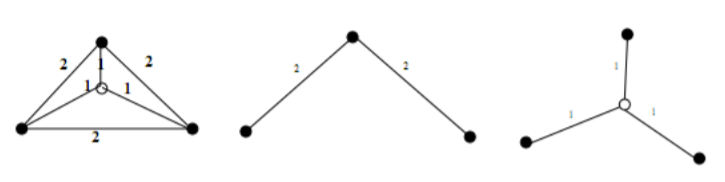
\includegraphics{img/steiner.png}
\caption{The first image shows the network topology. The black nodes are the
	target one. The second image is the result of a minimum spanning tree
	algorithm, which contains only the links that are involved as target
	nodes and it has a cost of 4. The third image shows the result of a
	minimum Steiner tree algorithm, which considers for the computation also
	non-target nodes to connect all the target nodes. Its cost is
	3}\label{fig:steiner}
\end{figure}

